\q{15}{Variable Elimination Algorithm Analysis}

Consider the variable elimination and enumeration algorithms:

{\bf function} ELIMINATION-ASK($X$, {\bf e}, $bn$) {\bf returns} a distribution over $X$\\
\indent\hspace{0.5cm}{\bf inputs}:\\
\indent\hspace{1.5cm}$X$, the query variable\\
\indent\hspace{1.5cm}{\bf e}, observed values for variables {\bf E}\\
\indent\hspace{1.5cm}$bn$, a Bayesian network specifying joint distribution {\bf P}$(X_1,...,X_n)$\\
\\\indent\hspace{0.5cm}$factors$ $\leftarrow$ {[}{]} \\
\indent\hspace{0.5cm}{\bf for each} $var$ {\bf in} ORDER($bn$.VARS) {\bf do}\\
\indent\hspace{1.0cm}$factors$ $\leftarrow$ {[}MAKE-FACTOR($var$, {\bf e}) $\mid$ $factors${]}\\
\indent\hspace{1.0cm}{\bf if} $var$ is a hidden variable {\bf then} $factors$ $\leftarrow$ SUM-OUT($var$, $factors$)\\
\indent\hspace{0.5cm}{\bf return} NORMALIZE(POINTWISE-PRODUCT($factors$))

\vspace{1cm}
{\bf function} ENUMERATION-ASK($X$, {\bf e}, $bn$) {\bf returns} a distribution over $X$\\
\indent\hspace{0.5cm}{\bf inputs}:\\
\indent\hspace{1.5cm}$X$, the query variable\\
\indent\hspace{1.5cm}{\bf e}, observed values for variables {\bf E}\\
\indent\hspace{1.5cm}$bn$, a Bayesian network specifying joint distribution {\bf P}$(X_1,...,X_n)$\\
\\\indent\hspace{0.5cm}{\bf Q}($X$) $\leftarrow$ a distribution over $X$, initially empty\\
\indent\hspace{0.5cm}{\bf for each} value $x_i$ of $X$ {\bf do}\\
\indent\hspace{1.0cm}{\bf Q}($x_i$) $\leftarrow$ ENUMERATE-ALL($bn$.VARS, {\bf e}$_{x_i}$)\\
\indent\hspace{1.5cm}where {\bf e}$_{x_i}$ is {\bf e} extended with $X = x_i$\\
\indent\hspace{0.5cm}{\bf return} NORMALIZE({\bf Q}($X$))\\

{\bf function} ENUMERATE-ALL($vars$, {\bf e}) {\bf returns} a real number\\
\indent\hspace{0.5cm}{\bf if} EMPTY?($vars$) {\bf then return} 1.0\\
\indent\hspace{0.5cm}$Y$ $\leftarrow$ FIRST($vars$)\\
\indent\hspace{0.5cm}{\bf if} $Y$ has value $y$ in {\bf e}\\
\indent\hspace{1.0cm}{\bf then return} $P(y \mid parents(Y))$ $\times$ ENUMERATE-ALL(REST($vars$), {\bf e})\\
\indent\hspace{1.0cm}{\bf else return} $\sum\nolimits_y P(y \mid parents(Y))$ $\times$ ENUMERATE-ALL(REST($vars$), {\bf e}$_y$)\\
\indent\hspace{1.5cm}where {\bf e}$_y$ is {\bf e} is extended with $Y = y$\\

\begin{figure}[h]
\centering
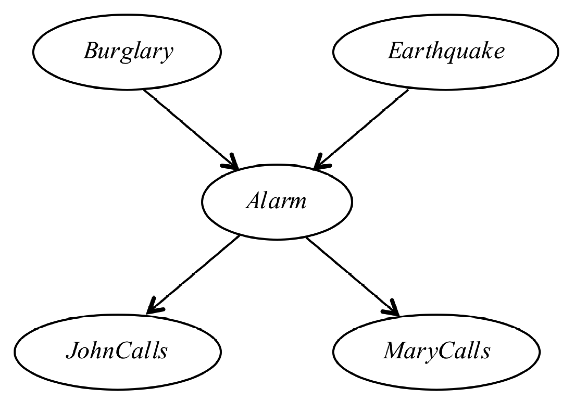
\includegraphics[width=0.4\linewidth]{figs/q3_burglary.png}
\end{figure}
\begin{question}{[5 pts]}
Count the number of arithmetic operations performed by the variable elimination algorithm on the query {\bf P}$(Burglary \mid JohnCalls = true, MaryCalls = true)$ and compare it with the number performed by the enumeration algorithm. Assume binary variables and the CPTs are given. 

\end{question}

13 operations for elimination (sum out E: 3, sum out A: 5, pointwise product: 2, normalization: 3). \\
31 operations for enumeration.

\vspace{1.5cm}

\begin{question}{[5 pts]}
Suppose a network has the form of a $chain$: a sequence of Boolean variables $X_1,...,X_n$ where $Parents(X_i) = \{X_{i-1}\}$ for $i=2,...,n$. What is the complexity of computing {\bf P}$(X_1 \mid X_n = true)$ using enumeration? Using variable elimination?
\end{question}
$O(n)$ for elimination because each variable eliminated requires only 3 operations to sum out\\
$O(2^n)$ for enumeration.
\vspace{1.5cm}

\begin{question}{[5 pts]}
Prove that the complexity of running variable elimination on a polytree network is linear in the size of the tree for any variable ordering consistent with the network structure (i.e. where the first variable eliminated will be a leaf node). {\em Hint}: use an induction on the number of nodes in the network.

\end{question}
% 
